\subsection[\textless{}T\textgreater]{Templates}

\begin{frame}[fragile]
  \frametitlecpp[17]{Templates}
  \begin{block}{Concept}
    \begin{itemize}
    \item The \cpp way to write reusable code
      \begin{itemize}
        \item like macros, but fully integrated into the type system
      \end{itemize}
    \item Applicable to functions, classes and variables
    \end{itemize}
  \end{block}
  \begin{cppcode}
    template<typename T>
    const T & max(const T &a, const T &b) {
      return b < a ? a : b;
    }
    template<typename T>
    struct Vector {
      int m_len;
      T* m_data;
    };
    template <typename T>
    std::size_t size = sizeof(T);
 \end{cppcode}
\end{frame}

\begin{frame}[fragile]
  \frametitlecpp[98]{Templates}
  \begin{alertblock}{Warning}
    \begin{itemize}
      \item they are compiled for each instantiation
      \item they need to be defined before used
      \begin{itemize}
        \item so all template code must typically be in headers
        \item or declared to be available externally (\mintinline{cpp}{extern template})
      \end{itemize}
      \item this may lead to longer compilation times and bigger binaries
    \end{itemize}
  \end{alertblock}
  \newsavebox{\codepiece}
  \begin{lrbox}{\codepiece}
    \begin{minipage}{.35\linewidth}
      \small
      \begin{cppcode*}{gobble=4}
        template<typename T>
        T func(T a) {
          return a;
        }
      \end{cppcode*}
    \end{minipage}
  \end{lrbox}
  \newsavebox{\codepiecea}
  \begin{lrbox}{\codepiecea}
    \begin{minipage}{.4\linewidth}
      \small
      \begin{cppcode*}{gobble=4,linenos=false}
        int func(int a) {
          return a;
        }
      \end{cppcode*}
    \end{minipage}
  \end{lrbox}
  \newsavebox{\codepieceb}
  \begin{lrbox}{\codepieceb}
    \begin{minipage}{.4\linewidth}
      \small
      \begin{cppcode*}{gobble=4,linenos=false}
        double func(double a) {
          return a;
        }
      \end{cppcode*}
    \end{minipage}
  \end{lrbox}
  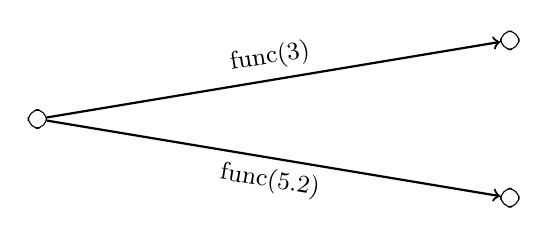
\begin{tikzpicture}[rectangle,rounded corners]
    \draw node (template) [draw] {\usebox{\codepiece}}
          node (templatea) [draw] at (6cm,+1cm) {\usebox{\codepiecea}}
          node (templateb) [draw] at (6cm,-1cm) {\usebox{\codepieceb}};
    \draw[->,thick] (template) -- (templatea) node [above,midway,sloped] {\small func(3)};
    \draw[->,thick] (template) -- (templateb) node [below,midway,sloped] {\small func(5.2)};
  \end{tikzpicture}
\end{frame}

\begin{frame}[fragile]
  \frametitlecpp[98]{Templates}
  \begin{block}{Template parameters}
    \begin{itemize}
    \item can be types, values or other templates
    \item you can have several
    \item default values allowed starting at the last parameter
    \end{itemize}
  \end{block}
  \begin{cppcode*}{}
    template<typename KeyType=int, typename ValueType=KeyType>
    struct Map {
      void set(const KeyType &key, ValueType value);
      ValueType get(const KeyType &key);
    };

    Map<std::string, int> m1;
    Map<float> m2;   // Map<float, float>
    Map<> m3;        // Map<int, int>
  \end{cppcode*}
\end{frame}

\begin{frame}[fragile]
  \frametitlecpp[98]{Template parameters}
  \begin{block}{\texttt{typename} vs. \texttt{class} keyword}
    \begin{itemize}
      \item for declaring a template type parameter,
            the \mintinline{cpp}{typename} and \mintinline{cpp}{class} keyword are semantically equivalent
      \item template template parameters required \cpp17 for \mintinline{cpp}{typename}
    \end{itemize}
  \end{block}
  \small
  \begin{cppcode*}{}
    template<typename T>
    T func(T a); // equivalent to:
    template<class T>
    T func(T a);

    template<template<class> class C>
    C<int> func(C<int> a); // equivalent to:
    template<template<typename> class C>
    C<int> func(C<int> a); // equivalent to:
    template<template<typename> typename C> // C++17
    C<int> func(C<int> a);
  \end{cppcode*}
\end{frame}

\begin{frame}[fragile]
  \frametitlecpp[98]{Template implementation}
  \begin{cppcode*}{}
    template<typename KeyType=int, typename ValueType=KeyType>
    struct Map {
      // declaration and inline definition
      void set(const KeyType &key, ValueType value) {
        ...
      }
      // just declaration
      ValueType get(const KeyType &key);
    };

    // out-of-line definition
    template<typename KeyType, typename ValueType>
    ValueType Map<KeyType, ValueType>::get
       (const KeyType &key) {
      ...
    }
  \end{cppcode*}
\end{frame}

\begin{frame}[fragile]
  \frametitle{Non-type template parameter \hfill \cpp98 / \cpp17 / \cpp20}
  \begin{block}{template parameters can also be values}
    \begin{itemize}
    \item integral types, pointer, enums in \cpp98
    \item \mintinline{cpp}{auto} in \cpp17
    \item literal types (includes floating points) in \cpp20
    \end{itemize}
  \end{block}
  \begin{cppcode*}{}
    template<unsigned int N>
    struct Polygon {
      Polygon(float radius);
      float perimeter() {return 2*N*sin(PI/N)*m_radius;}
      float m_radius;
    };

    Polygon<19> nonadecagon{3.3f};
  \end{cppcode*}
\end{frame}

\begin{frame}[fragile]
  \frametitlecpp[98]{Template specialization}
  \begin{block}{Specialization}
    Templates can be specialized for given values of their parameter
  \end{block}
  \small
  \begin{cppcode*}{}
    template<typename F, unsigned int N>
    struct Polygon { ... }; // primary template

    template<typename F> // partial specialization
    struct Polygon<F, 6> {
      Polygon(F radius) : m_radius(radius) {}
      F perimeter() { return 6*m_radius; }
      F m_radius;
    };
    template<>           // full specialization
    struct Polygon<int, 6> {
      Polygon(int radius) : m_radius(radius) {}
      int perimeter() { return 6*m_radius; }
      int m_radius;
    };
  \end{cppcode*}
\end{frame}

\begin{advanced}

\begin{frame}[fragile]
  \frametitlecpp[98]{Template argument deduction}
  \begin{block}{Template argument deduction}
    \begin{itemize}
    \item Template arguments deduced from (function) arguments
    \item Template arguments can always be specified explicitly
    \item Only for function templates (Before \cpp14)
    \end{itemize}
  \end{block}
  \begin{cppcode*}{}
    template <typename T, typename U>
    void f(T t, U u) { ... }

    f(42, true);        // deduces T=int, U=bool
                        // calls f<int, bool>(42, true);
    f<float>(42, true); // sets T=float, deduces U=bool
                        // calls f<float, bool>(42, true);
                        // 42 converted to float before call
  \end{cppcode*}
\end{frame}

\begin{frame}[fragile]
  \frametitlecpp[11]{Template argument deduction}
  \begin{block}{Deduced contexts}
    \begin{itemize}
    \item Compiler can even deduce template arguments inside certain expressions (pattern matching)
    \item See \href{https://en.cppreference.com/w/cpp/language/template_argument_deduction}{cppreference} for details
    \end{itemize}
  \end{block}
  \begin{cppcode*}{}
    template <typename T>
    void f(T* p) { ... }

    const int * ip = ...;
    f(ip); // deduces T=const int

    template <typename T, std::size_t N>
    void g(std::array<T*, N> a) { ... }

    std::array<int*, 3> aip = ...;
    g(aip); // deduces T=int, N=3
  \end{cppcode*}
\end{frame}

\begin{frame}[fragile]
  \frametitlecpp[11]{Template argument deduction}
  \begin{block}{Non-deduced contexts}
    \begin{itemize}
    \item Deduction from certain expressions is impossible/forbidden
    \end{itemize}
  \end{block}
  \begin{overprint}
    \onslide<1>
    \begin{alertblock}{}
      \footnotesize
      \begin{cppcode*}{gobble=2}
        template <typename C>
        void f(typename C::value_type v) { ... }
        f(std::vector<int>{...}); // cannot deduce C
                                  // from a dependent type
        template <typename T, std::size_t N>
        void g(std::array<T, N * 2> a) { ... }
        g(std::array<int, 4>{...}); // deduces T=int,
                                    // cannot deduce N from expression
        template <typename T>
        void h(std::vector<T> v) { ... }
        h({1, 2, 3}); // error, braced-initializer list has no type
        h(std::vector<int>{1, 2, 3}); // ok, T=int
      \end{cppcode*}
    \end{alertblock}
    \onslide<2>
    \begin{alertblock}{}
      \footnotesize
      \begin{cppcode*}{gobble=2}
        template <typename C, typename F>
        void reduce(const C& cont, const F& f = std::plus{});
        reduce(std::vector<int>{...}); // error: cannot deduce F
        // would need: <typename C, typename F = decltype(std::plus{})>

        template<typename T>
        const T & max(const T &a, const T &b) { ... }
        int i = 3;
        max(i, 3.14f); // deduces T=int and T=float, error
        // either: max<float>(i, 3.14f);
        // or:     max(static_cast<float>(i), 3.14f);
      \end{cppcode*}
    \end{alertblock}
  \end{overprint}
\end{frame}

\begin{frame}[fragile]
  \frametitlecpp[11]{Template argument deduction}
  \begin{block}{Deduction in partial specializations}
    \begin{itemize}
      \item Partial specializations also deduce template arguments
      \begin{itemize}
        \item with similar rules as for function templates
        \item but some more restrictions (cf.\ \href{https://en.cppreference.com/w/cpp/language/partial_specialization}{cppreference})
      \end{itemize}
    \end{itemize}
  \end{block}
  \small
  \begin{cppcode*}{}
    template <typename T>
    struct S { ... }; // primary template

    template <typename T>
    struct S<T*> { ... }; // specialization 1

    template <typename T, std::size_t N>
    struct S<std::array<T*, N>> { ... }; // specialization 2

    S<int>  s1; // prim. tmpl. (T=int) ok, spec. 1/2 invalid
    S<int*> s2; // prim. tmpl. (T=int*) and spec. 1 (T=int) ok
                // spec. 1 is more specialized, will be used
  \end{cppcode*}
\end{frame}

\begin{frame}[fragile]
  \frametitlecpp[98]{Template argument deduction}
  \begin{block}{Specialization vs.\ overloading}
    \begin{itemize}
      \item For function templates we can choose between specialization and overloading
      \item Partial specialization of function templates is forbidden
    \end{itemize}
  \end{block}
  \small
  \begin{multicols}{2}
    \begin{cppcode*}{}
      template <typename T>
      void f(T t) { ... }


      void f(int* t) { ... }


      template <typename T>
      void f(T* t) { ... }
    \end{cppcode*}
    \columnbreak
    \begin{cppcode*}{}
      template <typename T>
      void f(T t) { ... }

      template <>
      void f<int*>(int* t) { ... }

      // part. spec. forbidden:
      template <typename T>
      void f<T*>(T* t) {...}
    \end{cppcode*}
  \end{multicols}
\end{frame}

\begin{frame}[fragile]
  \frametitlecpp[11]{Template argument deduction}
  \begin{block}{Disadvantages of specialization vs.\ overloading}
    \begin{itemize}
      \item Specialization always needs a primary template
      \begin{itemize}
        \item Sometimes this does not make sense
      \end{itemize}
      \item Partial specializations of function templates is forbidden
      \begin{itemize}
        \item So we need SFINAE workarounds or concepts
      \end{itemize}
    \end{itemize}
  \end{block}
  \small
  \begin{block}{Could you express this with specializations?}
    \begin{cppcode}
      template <typename T>
      void f(T* p) { ... }

      template <typename T>
      void f(std::unique_ptr<T> p) { ... }
    \end{cppcode}
  \end{block}
  \begin{goodpractice}{Specialization vs.\ overloading}
    Prefer overloading function templates over template specialization
  \end{goodpractice}
\end{frame}

\begin{frame}[fragile]
  \frametitlecpp[17]{Class Template Argument Deduction (CTAD)}
  \begin{block}{CTAD}
    \begin{itemize}
    \item Deduce the template arguments for a class template
    \item Based on construction arguments
    \item Only when no template arguments provided
    \item Since \cpp20: CTAD for aggregates (no constructor needed)
    \end{itemize}
  \end{block}
  \begin{cppcode*}{}
    template<typename A, typename B, typename C = double>
    struct Triple {
      Triple(A a, B b, C c) : a(a), b(b), c(c) {} // C++17
      A a; B b; C c;
    };

    Triple t{42, true, 3.14}; // Triple<int, bool, double>
    Triple<int> t{42, true, 3.14}; // compilation error
    Triple<int, bool> t{42, true, 3.14}; // not CTAD
  \end{cppcode*}
\end{frame}

\begin{frame}[fragile]
  \frametitlecpp[17]{Class Template Argument Deduction (CTAD)}
  \begin{block}{Deduction guides}
    \begin{itemize}
    \item Describe how constructor argument types are mapped to class template arguments
    \end{itemize}
  \end{block}
  \begin{cppcode}
    template<typename A, typename B>
    struct Pair {
     Pair(A a, B b) : a(a), b(b) {}
     A a; B b;
    };
  \end{cppcode}
  \begin{overprint}[\columnwidth]
    \onslide<1>
    \begin{cppcode*}{gobble=2,firstnumber=6}



      Pair p{42, "hello"}; // Pair<int, const char*>
    \end{cppcode*}
    \onslide<2>
    \begin{cppcode*}{gobble=2,firstnumber=6}
      template<typename A>
      Pair(A, const char*) -> Pair<A, std::string>;

      Pair p{42, "hello"}; // Pair<int, std::string>
    \end{cppcode*}
  \end{overprint}
\end{frame}

\begin{frame}[fragile]
  \frametitlecpp[17]{Class Template Argument Deduction (CTAD)}
  \begin{block}{Standard library examples}
    \begin{cppcode*}{gobble=2}
      std::pair p{1.2, true}; // std::pair<double, bool>
      std::tuple t{1.2, true, 32};
                        // std::tuple<double, bool, int>
      std::vector v{1, 2, 3}; // std::vector<int>
      std::list l{v.begin(), v.end()}; // std::list<int>
      std::array a{1, 2, 3}; // std::array<int, 3>

      std::mutex m;
      std::lock_guard l(m); // std::lock_guard<std::mutex>
    \end{cppcode*}
  \end{block}
\end{frame}

\end{advanced}

\begin{frame}[fragile]
  \frametitlecpp[98]{The full power of templates}
  \begin{exercise}{Templates}
    \begin{itemize}
    \item go to code/templates
    \item look at the OrderedVector code
    \item compile and run playwithsort.cpp. See the ordering
    \item modify playwithsort.cpp and reuse OrderedVector with Complex
    \item improve OrderedVector to template the ordering
    \item test reverse ordering of strings (from the last letter)
    \item test order based on {\color{blue} \href{https://en.wikipedia.org/wiki/Taxicab_geometry}{Manhattan distance}} with complex type
    \item check the implementation of Complex
    \item try ordering complex of complex
    \end{itemize}
  \end{exercise}
\end{frame}
